\documentclass[pra,12pt]{revtex4}
\usepackage{amsmath}
\usepackage{amssymb}
\usepackage{graphicx}
\usepackage{color}
\usepackage[pdfborder={0 0 0},colorlinks=true,linkcolor=blue]{hyperref}

\def\ket#1{\left|#1\right\rangle}
\def\bra#1{\left\langle#1\right|}
\def\braket#1{\left\langle#1\right\rangle}

\setlength{\parindent}{0pt}

\renewcommand{\baselinestretch}{1.0}
\setlength{\parskip}{0.07in}

\begin{document}

\section{Bound states and extended states}

One of the most interesting features of wavefunctions in infinite
space is that they come in two distinct types: (i) \textbf{extended
  states}, which spread out over the entire space, and (ii)
\textbf{bound states}, which are localized in one region.  Both types
can co-exist in a single system.

The \textbf{1D finite square well} is a simple model which exhibits
both bound and extended states.  Consider the Hamiltonian
$$\hat{H} = \frac{\hat{p}^2}{2m} - V_0 \,\Theta(a -|\hat{x}|),$$ where
$\hat{x}$ and $\hat{p}$ are the 1D position and momentum operators,
$m$ is the particle mass, $V_0$ and $a$ are positive real parameters,
and $\Theta(\cdots)$ denotes the Heaviside step function (which is 1
if the input is positive, and 0 otherwise).  The potential describes a
square well of depth $V_0$ and width $2a$.  Inside the well region
($|x| < a$), the potential is $-V_0$; outside, it is zero.

\begin{figure}[h]
  \centering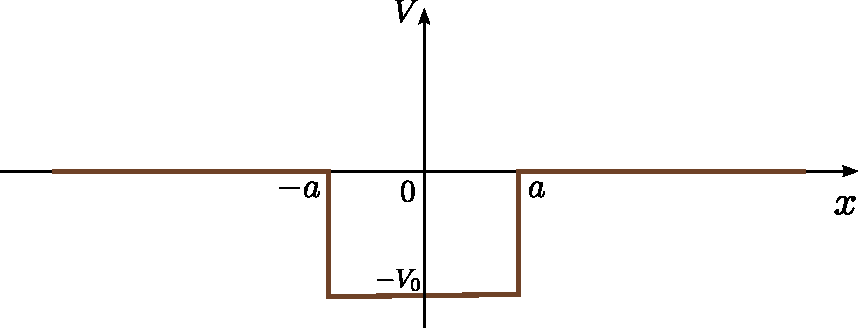
\includegraphics[width=0.7\textwidth]{squarewell}
\end{figure}

We wish to solve the time-independent Schr\"odinger equation for this
Hamiltonian.  In \hyperref[sec:appendix]{Appendix A}, we describe a
common numerical method, known as the \textbf{transfer matrix method},
which can be used to generate solutions for the square well and other
similar 1D potentials.  In this section, we not deal with the
calculation details, but instead zoom in on certain key facts.

The first thing to note is that when solving the Schr\"odinger wave
equation, it's necessary to specify the boundary conditions at
infinity.  This choice affects whether we get a bound state or
extended state.  The wavefunction of a bound state diminishes
exponentially as $x \rightarrow \pm\infty$; thus, in either external
region (i.e., $x < -a$ or $x > a$), it satisfies
$$-\frac{\hbar^2}{2m}\,\frac{d^2\psi}{dx^2} = E \psi(x),$$
subject to the boundary conditions
$$\psi(x) \overset{x\rightarrow\pm\infty}{\sim} e^{\mp\kappa x}, \;\;\;\mathrm{Re}(\kappa) > 0.$$
The bound state solutions in the external regions therefore take the
form
$$\psi(x) = c_\pm\, e^{\mp\kappa x}, \;\;\mathrm{where}\;\, -\frac{\hbar^2\kappa^2}{2m} = E, \;\; c_\pm \in \mathbb{C}.$$
Since $E$ is real, it follows that $\kappa$ is real, and hence $E <
0$.  Moreover, the variational principle implies that $E \ge -V_0$.
Hence, bound state energies are restricted to the range $-V_0 \le E <
0$.  We can also show that the bound state energies are
\textit{discrete}: the energy spacing decreases with $a$, but so long
as $a$ is finite, the spacing is non-vanishing.  Another related
fact is that the wavefunction for a bound state can always be
normalized:
$$\int_{-\infty}^\infty |\psi(x)|^2\, dx\; =\; 1.$$
The normalization integral will not diverge, as $|\psi(x)|^2$ vanishes
exponentially as $x \rightarrow \pm \infty$.

For an extended state, the situation is quite different.  In this
case, the wavefunction does not vanish exponentially at infinity, but
instead takes the form
$$\psi(x) = \begin{cases} \alpha_-\, e^{ik x} + \beta_-\, e^{-ik x}, & \;\;\;x < -a\\ (\mathrm{something}) , & -a < x < a\\ \alpha_+\, e^{ik x} + \beta_+\, e^{-ik x} , & \;\;\,x > a.\end{cases}$$
Within each external region, $\psi(x)$ consists of a superposition of
left-moving and right-moving plane waves, with wavenumber $k$.  The
coefficients $\alpha_\pm$ and $\beta_\pm$ are not independent
quantities, but are linked by a linear relation (see
\hyperref[sec:appendix]{Appendix A}).  In order to satisfy
Schr\"odinger's equation, $k$ must satisfy
$$\frac{\hbar^2k^2}{2m} = E,$$
which means that extended states occur only for energies $E \ge 0$.
In fact, the solutions form a continuum, meaning we can find extended
states for \textit{every} $E \ge 0$.  Since $|\psi(x)|^2$ does not
diminish exponentially at infinity, the integral $\int_{-\infty}^\infty
|\psi(x)|^2\, dx$ necessarily diverges.  Hence, the wavefunction
has no finite normalization.  (Note: we formally exclude the case of
wavefunctions that blow up at infinity, rather than going to a
constant magnitude.  To understand why, and for a more rigorous
discussion of how extended states are normalized, see
\hyperref[sec:normalization]{Appendix B}.)

The following figure shows numerically-obtained results for a square
well with $V_0 = 30$ and $a=1$ (in units where $\hbar = m =1$).  The
energy spectrum is shown on the left side.  There exist five bound
states; their plots of $|\psi|^2$ versus $x$ are shown on the right
side.  These results were computed using the transfer matrix code
described in \hyperref[sec:appendix]{Appendix A}.

\begin{figure}[h]
  \centering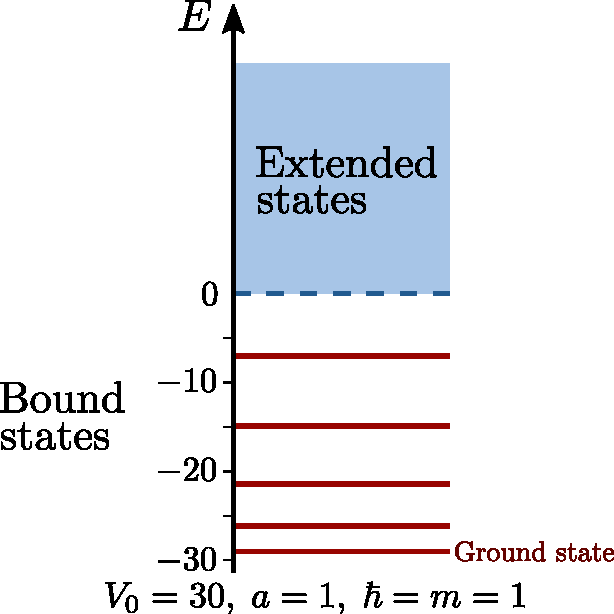
\includegraphics[width=0.81\textwidth]{boundvsextended}
\end{figure}

%% For $E \ge 0$, there is a continuum of extended states, which do not
%% have any finite normalization.  For $-V_0 < E < 0$, which is the
%% energy range ``inside'' the potential well, there exists a discrete
%% and finite set of bound states, whose wavefunctions vanish
%% exponentially outside the well and are therefore normalizable.

Many of the lessons drawn from this square well model can be
generalized to more complicated potential wells.  (Also, in cases
where the potential at infinity is $V_{\textrm{ext}}$ rather than
zero, extended states occur for $E \ge V_{\textrm{ext}}$ and bound
states occur for $\textrm{min}(V) < E < V_{\textrm{ext}}$.)

There are, however, two important provisos to bear in mind.  The first
is that if we vary the potential, the number of bound states can
change: i.e., bound state solutions can either appear or disappear.  A
numerical example is given below, showing the bound state energies for
the square well model with fixed $a = 1$ and varying well depth $V_0$:

\begin{figure}[h]
  \centering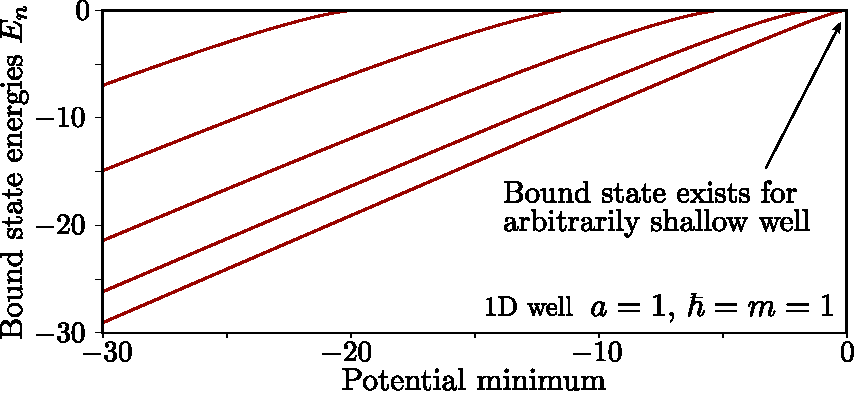
\includegraphics[width=0.65\textwidth]{boundstate1d}
\end{figure}

For $V_0 = 30$, there are five bound states, but these disappear one
by one as we make the potential well shallower.  Note, however, that
one bound state survives in the limit $V_0 \rightarrow 0$.  There is a
theorem which states that any 1D attractive potential, no matter how
weak, always supports at least one bound state.  For details, see
\hyperref[ex:boundstate]{Exercise 1}.

In 3D, however, it is possible for an attractive potential to be ``too
weak'' to support a bound state.  Intuitively, this happens if the
zero-point energy of any prospective ground state exceeds the well
depth.  A numerical example is given below, for a uniform
spherically-symmetric well in 3D (the $l$'s label the angular momentum
quantum numbers).  For details, see
\hyperref[ex:boundstate3d]{Exercise 2}.

\begin{figure}[h]
  \centering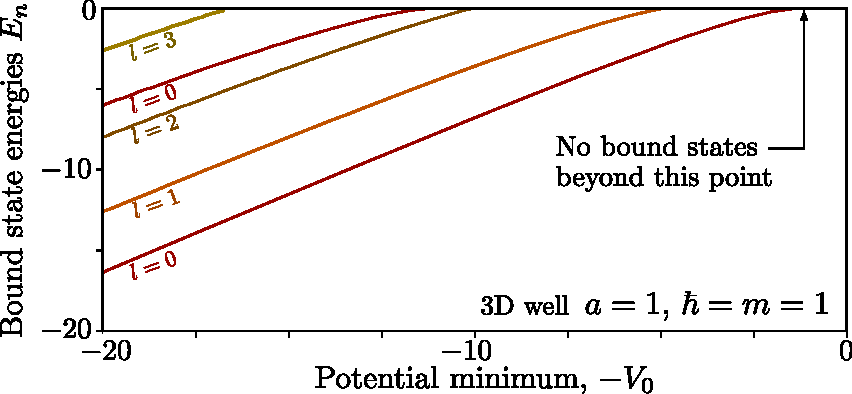
\includegraphics[width=0.65\textwidth]{boundstate3d}
\end{figure}

Another proviso to keep in mind is that in certain cases, it is
actually possible to have bound states with energy $E \ge 0$.  These
are called ``bound states in the continuum'', since they lie in the
same energy range as the continuum of extended states.  We will ignore
this phenomenon, since it happens only under special circumstances
that lie outside the scope of the present discussion.  The interested
reader may refer to the review by \hyperref[cite:hsu]{Hsu \textit{et
    al.}~(2016)}.

\section{Quasi-bound states and resonances}

For the 1D finite square well, bound states and extended states behave
very differently from each other.  In certain other models, however,
extended states can take on characteristics similar to bound states.
These are called \textbf{quasi-bound states}, and they play an
especially important role in scattering experiments.

An example of a potential function $V(x)$ that supports quasi-bound
states is shown below.  In the external regions, $|x| > b$, the
potential is zero.  Between $x = -b$ and $x = b$, sits a ``barrier''
of positive potential $V_1$.  Embedded in the middle of this barrier,
in the region $|x| < a$, is a central well of potential $V_0$ such
that $0 < V_0 < V_1$.

\begin{figure}[h]
  \centering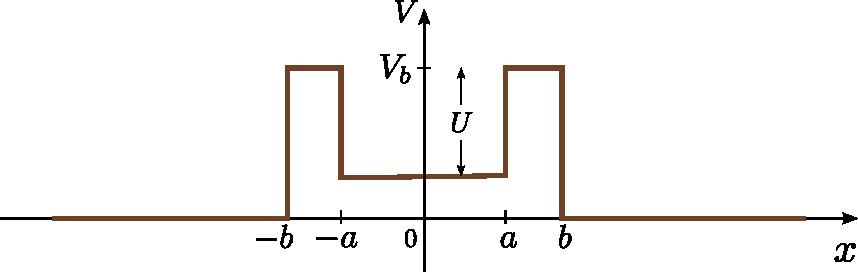
\includegraphics[width=0.7\textwidth]{resonancewell}
\end{figure}

This potential is purely repulsive, so the discussion in the previous
section tells us there are no bound states, only extended states.

However, there's something intriguing about the energy range
corresponding to the central well, $V_0 < E < V_1$.  Consider a
slightly different situation, where the potential in the exterior
region is $V_1$ rather than $0$; i.e., the potential function is a
finite square well:
$$V_{\mathrm{alt}}(x) = \begin{cases}V_0, & |x| < a, \\ V_1, & \mathrm{otherwise}.\end{cases}$$
In this case, there will be bound states somewhere in the energy range
$V_0 < E < V_1$.  These bound states' wavefunctions diminish
exponentially away from the square well, and are thus close to zero
for $|x| > b$.  But since $V(x)$ and $V_{\mathrm{alt}}(x)$ differ from
each other only in the region $|x| > b$, these wavefunctions ought to
act as \textit{approximate} solutions to the Schr\"odinger wave
equation for the original potential function $V(x)$---which does not
support bound states!

Turning this argument around, we expect the potential function $V(x)$
to support certain extended states whose wavefunctions look very
similar to bound states, but aren't bound.

To find evidence of quasi-bound states, let us analyze the system
using the framework of a \textbf{scattering experiment}, as developed
in the previous chapter.  Let a particle be incident from the left,
with energy $E > 0$, described by the incident wavefunction
$$\psi_i(x) = \Psi_i \, e^{ik_i x}.$$
This gives rise to a scattered wavefunction $\psi_s(x)$, such that the
total wavefunction $\psi_i(x) + \psi_s(x)$ satisfies the Schr\"odinger
wave equation with energy $E$.  The scattered wavefunction must be
outgoing (see the previous chapter), so in the external region it
takes the form
$$\psi_s(x) = \Psi_i \times \begin{cases}f_- \,e^{-ik_ix}, & x \le -b \\ f_+ \,e^{ik_ix}, & x \ge b.\end{cases}$$
The scattering amplitudes $f_+$ and $f_-$ can be found by solving the
Schr\"odinger wave equation, using the transfer matrix method
described in \hyperref[sec:appendix]{Appendix A}.  The figure below
shows numerical results obtained for $V_0 = 10,\,V_1 = 30,\,a=1$, and
$b = 1.2$ or $b = 1.4$, with $\hbar = m = 1$.

\begin{figure}[h]
  \centering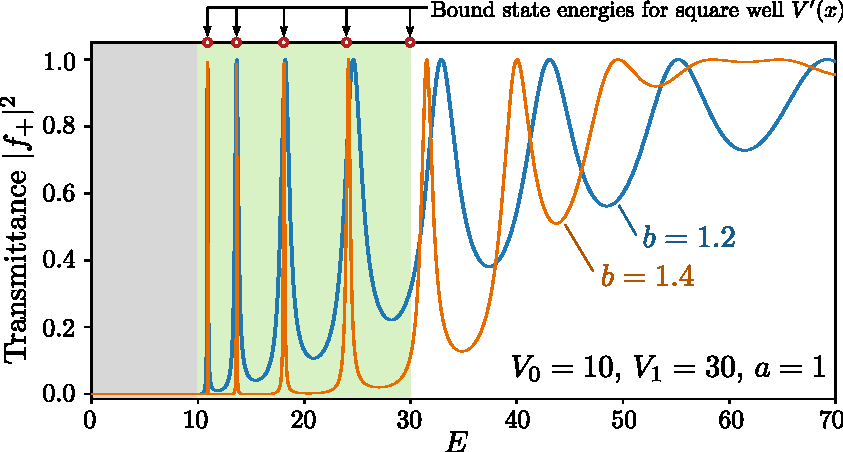
\includegraphics[width=0.65\textwidth]{resonances}
\end{figure}

The vertical axis shows $|f_+|^2$, which is called the
``transmittance'' and measures the probability for the incident
particle to pass through the potential.  The horizontal axis is the
particle energy $E$.  For $E < V_0$, the transmittance approaches
zero, and for $E \gtrsim V_1$, the transmittance approaches unity, as
expected.  Within the energy range $V_0 < E \lesssim V_1$, the
transmittance forms a series of narrow peaks, which get sharper for
larger $b$ (i.e., when the central well is more isolated from the
exterior space).  At the top of the figure, we have also plotted the
bound state energies for the square well potential $V'(x)$, which
closely matches the energies of the transmittance peaks (at least, the
first four peaks).

Upon examining the total wavefunction $\psi(x)$ at these special
energies, we see something very interesting.  The figure below plots
$|\psi(x)|^2$ versus $x$ at the energies corresponding to the first
three transmittance peaks, along with the bound state wavefunctions
for the corresponding square well model.  We find that $|\psi(x)|^2$
is much larger within the potential region than the exterior region.
Moreover, its profile is very similar to the corresponding bound
state.

\textcolor{red}{[Fig.]}

The enhancement of $|\psi(x)|^2$ is called a \textbf{resonance}.  It
happens because the system has a quasi-bound state (an extended state)
that is very similar to a bound state of a closely-related system
(which is localized to the well region).  This phenomenon is closely
analogous to resonances occurring in classical mechanics.  If we take
a classical system with a natural oscillation frequency, such as a
damped harmonic oscillator, and drive it at a fixed frequency, the
oscillation amplitude becomes extremely large when the driving
frequency matches the natural oscillation frequency.

Resonances play a critical role throughout experimental physics.
Experiments are often conducted for the express purpose of locating
and studying resonances.  When a resonance-induced scattering peak is
found, the location and shape of the peak can be used to deduce
various important features of the quasi-bound state, which often
provides a great deal of important information about the system
itself.

\section{General analysis of scattering resonances}

Quasi-bound states and scattering resonances are not limited to 1D;
they are equally important, if not more so, in 2D and 3D systems.  The
Green's function operator, introduced in the previous chapter,
provides a convenient and general way to study them.



\section{Decay rate of a quasi-bound state: Fermi's Golden Rule}

\section{The decay spectrum of beta particles}


\appendix
\section{The transfer matrix method}
\label{sec:appendix}


\section{Normalization of bound states and extended states}
\label{sec:normalization}

In this Appendix, we take a closer look at where bound and extended
states come from, and how they are normalized.  Imagine that instead
of taking $x \in (-\infty,\infty)$, we enclose the system in a very
large but finite box, so that $x \in [-L,L]$ where $L \gg a$.  We
impose periodic boundary conditions on the box walls, $\psi(-L) \equiv
\psi(L)$, and solve the Schr\"odinger equation for wavefunctions
normalizable within the box, such that $\int_{-L}^{L} |\psi(x)|^2 dx =
1$.  For any finite $L$, there is an infinite but discrete set of
solutions, with energies in the range $-V_0 <E < \infty$.

We now examine how the solutions vary upon increasing $L$.

\textcolor{red}{[Fig.]}





\section*{Exercises}

\begin{enumerate}
\item Existence of bound states in 1D
\label{ex:boundstate}

\item In this problem, you will investigate the existence of bound
  states in a 3D potential well that is finite, uniform, and
  spherically-symmetric.  The potential function is
$$V(r,\theta,\phi) = -V_0\Theta(a-r),$$
  where $a$ is the radius of the spherical well, $V_0$ is the depth,
  and $(r,\theta,\phi)$ are spherical coordinates defined in the usual
  way.  For $E < 0$, the Schr\"odinger equation reduces to
$$\begin{cases}\Big(\nabla^2 + q^2\Big) \psi(r,\theta,\phi) = 0 \;\;\mathrm{where}\;\; q = \sqrt{2m(E+V_0)/\hbar^2}, \;\;&\mathrm{for} \; r \le a \\ \Big(\nabla^2 - \gamma^2\Big) \psi(r,\theta,\phi) = 0 \;\;\mathrm{where}\;\; \gamma = \sqrt{-2mE/\hbar^2}, \;\;&\mathrm{for} \; r \ge a. \end{cases}$$
  For the first equation (called the Helmholtz equation), we seek
  solutions of the form
  $$\psi(r,\theta,\phi) = f(r) \, Y_{lm}(\theta,\phi),$$
  where $Y_{lm}(\theta,\phi)$ are
  \href{https://en.wikipedia.org/wiki/Spherical_harmonics}{spherical
    harmonics}; the integers $l$ and $m$ are angular momentum
  quantum numbers satisfying $l \ge 0$ and $-l \le m \le l$.
  Substituting this into the Helmholtz equation gives
  $$r^2\frac{d^2f}{dr^2} + 2r \frac{df}{dr}+\left[q^2r^2-l(l+1)\right] f(r) = 0,$$
  which is the \textbf{spherical Bessel equation}.  The set of
  solutions that are non-divergent at $r = 0$ are $f(r) = j_l(qr)$,
  where $j_l$ is called a \textbf{spherical Bessel function of the
    first kind}.  Most numerical packages provide functions to
  calculate these (e.g.,
  \href{https://docs.scipy.org/doc/scipy/reference/generated/scipy.special.spherical_jn.html}{\texttt{scipy.special.spherical\_jn}}
  in Scientific Python).

  Similarly, solutions for the second equation can be written as
  $\psi(r,\theta,\phi) = g(r) \, Y_{lm}(\theta,\phi),$ yielding an
  equation for $g(r)$ called the \textbf{modified spherical Bessel
    equation}.  The solutions which do not diverge as $r\rightarrow
  \infty$ are $g(r) = k_l(\gamma r)$, where $k_l$ is called a
  \textbf{modified spherical Bessel function of the second kind}.
  Again, this can be computed numerically (e.g., using
  \href{https://docs.scipy.org/doc/scipy/reference/generated/scipy.special.spherical_kn.html#scipy.special.spherical_kn}{\texttt{scipy.special.spherical\_kn}}
  in Scientific Python).

  Using the above facts, show that the condition for a bound state to
  exist is
  $$\frac{qj_l'(qa)}{j_l(qa)} = \frac{\gamma k_l'(\gamma a)}{k_l(\gamma a)},$$
  where $j_l'$ and $k_l'$ denote the derivatives of the relevant
  special functions, and $q$ and $\gamma$ depend on $E$ and $V_0$ as
  described above.  Write a program to search for the bound state
  energies at any given $a$ and $V_0$, and hence determine the
  conditions under which the potential does not support bound
  states.



\label{ex:boundstate3d}

\item Phase shift under scattering resonance

\item Classical driven oscillator analogy  
\end{enumerate}




\section*{Further Reading}

\begin{itemize}
\item Bransden \& Joachain, \S4.4, 9.2--9.3, 13.4
\item Sakurai, \S5.6, 7.7--7.8

\end{itemize}

\section*{Further Reading}

\begin{itemize}
\item 
  C.~W.~Hsu, B.~Zhen, A.~D.~Stone, J.~D.~Joannopoulos, and
  M.~Solja\u{c}i\'{c}, \textit{Bound states in the continuum},
  Nature Reviews Materials \textbf{1}, 16048 (2016).
  \label{cite:hsu}
\end{itemize}

\end{document}


%% For decades after the discovery of quantum mechanics, the quantum
%% double-slit experiment was just a ``thought experiment'', meant to
%% illustrate the features of quantum mechanics that had been uncovered
%% by other, more complicated experiments.  Nowadays, the most convenient
%% way to do the experiment is with light, using single-photon sources
%% and single-photon detectors.  Quantum interference has also been
%% demonstrated experimentally using electrons, neutrons, and even
%% large-scale particles such as buckyballs.
